\chapter{KẾT QUẢ THỰC NGHIỆM VÀ SO SÁNH}

Chương này trình bày kết quả của bảy thí nghiệm E0--E6. Quy ước đọc số liệu: cột \textbf{CV F1} là F1 của lớp spam trung bình qua kiểm định chéo 5 fold \textit{chỉ trên tập huấn luyện} và là căn cứ chọn mô hình; các cột \textbf{Test} được tính trên tập kiểm tra giữ riêng (1\,032 tin, trong đó 128 spam) và chỉ dùng để báo cáo.

\section{Kết quả tổng hợp}

\begin{table}[H]
\centering
\caption{Kết quả của các thí nghiệm trên tập kiểm tra ($\text{spam}$ là lớp dương)}
\label{tab:ket-qua}
\small
\begin{tabular}{|c|c|c|c|c|c|c|c|}
\hline
\textbf{ID} & \textbf{CV F1} & \textbf{Acc.} & \textbf{Prec.} & \textbf{Recall} & \textbf{F1} & \textbf{AUC} & \textbf{TN/FP/FN/TP} \\
\hline
E0 (baseline) & 0,9385 & 0,9826 & 0,9508 & 0,9062 & 0,9280 & 0,9790 & 898/6/12/116 \\
\hline
E1 & 0,8512 & 0,9719 & 0,9901 & 0,7812 & 0,8734 & 0,9832 & 903/1/28/100 \\
\hline
E2 & 0,9365 & 0,9845 & 0,9746 & 0,8984 & 0,9350 & 0,9882 & 901/3/13/115 \\
\hline
E3 (K-NN) & 0,8935 & 0,9758 & 0,9640 & 0,8359 & 0,8954 & 0,9685 & 900/4/21/107 \\
\hline
E4 (Cây) & 0,8086 & 0,9700 & 0,9450 & 0,8047 & 0,8692 & 0,8954 & 898/6/25/103 \\
\hline
\textbf{E5} & \textbf{0,9425} & \textbf{0,9864} & 0,9750 & \textbf{0,9141} & \textbf{0,9435} & 0,9905 & 901/3/11/117 \\
\hline
E6 & 0,9283 & 0,9845 & 0,9746 & 0,8984 & 0,9350 & 0,9920 & 901/3/13/115 \\
\hline
\end{tabular}
\Nguon{Nhóm tổng hợp từ tệp \texttt{outputs/results/metrics.csv}}
\end{table}

Theo tiêu chí đã đặt trước (CV F1), \textbf{E5 là cấu hình tốt nhất}: Accuracy 98,64\%, Precision 97,50\%, Recall 91,41\%, F1 94,35\%, ROC-AUC 0,9905. Trên 1\,032 tin kiểm tra mô hình chặn nhầm 3 tin hợp lệ và bỏ lọt 11 tin spam.

Ma trận nhầm lẫn chi tiết của E5 nằm ở Phụ lục 2 (Hình~\ref{fig:cm-e5}).

\begin{figure}[H]
    \centering
    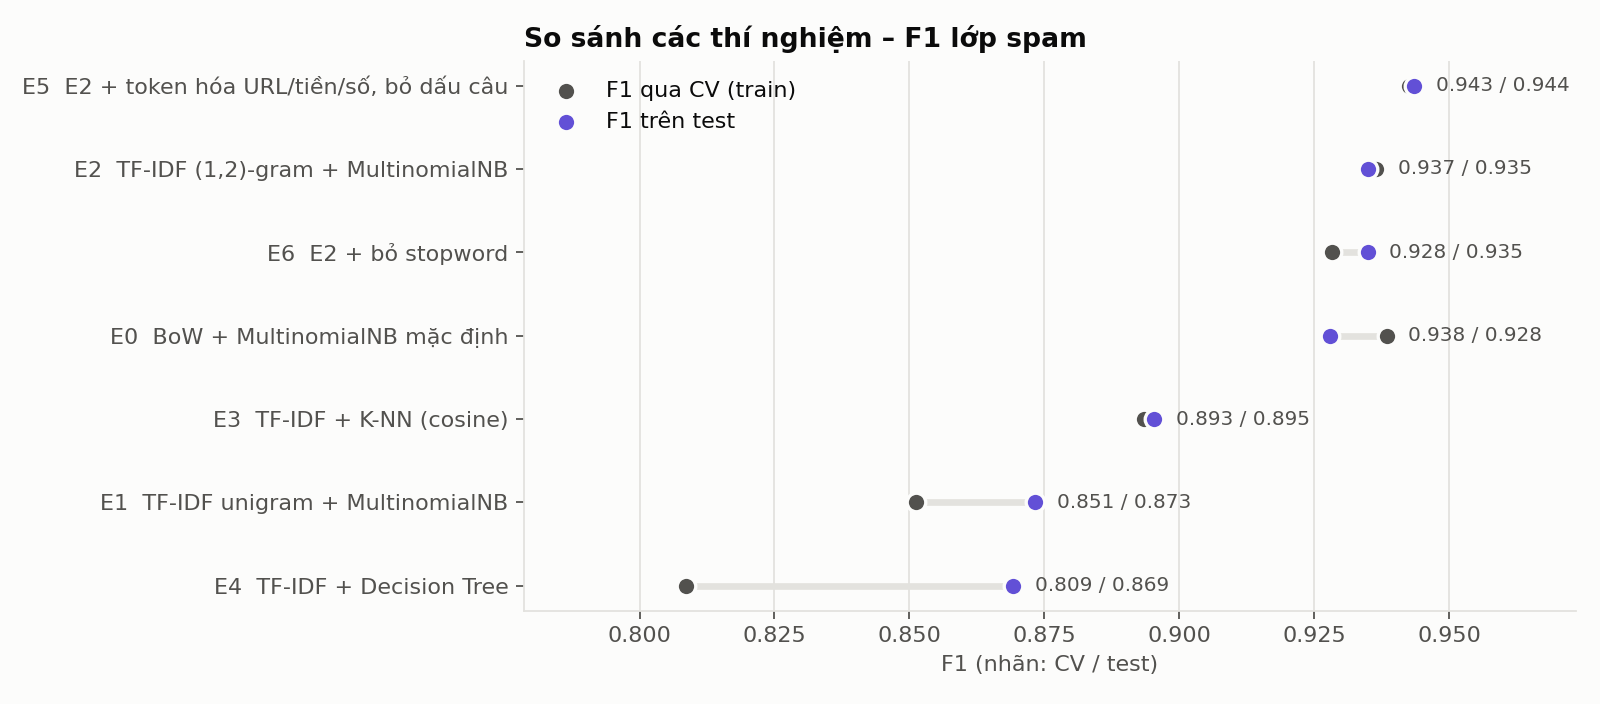
\includegraphics[width=\textwidth]{images/viz_3_model_comparison.png}
    \caption{So sánh F1 của lớp spam giữa kiểm định chéo (chấm đen) và tập kiểm tra (chấm tím)}
    \label{fig:so-sanh-mo-hinh}
    \Nguon{Nhóm xây dựng từ kết quả thí nghiệm}
\end{figure}

\begin{figure}[H]
    \centering
    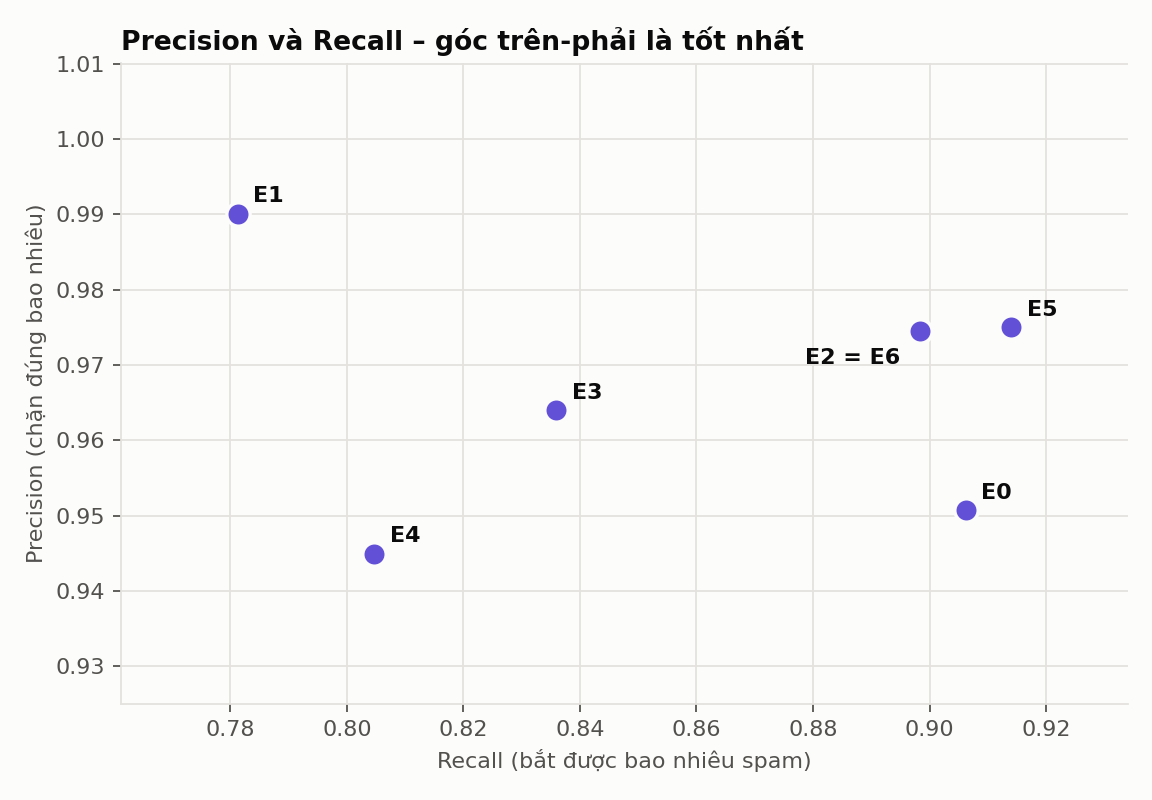
\includegraphics[width=0.78\textwidth]{images/viz_4_precision_recall.png}
    \caption{Precision và Recall của các thí nghiệm trên tập kiểm tra}
    \label{fig:precision-recall}
    \Nguon{Nhóm xây dựng từ kết quả thí nghiệm}
\end{figure}

\subsection{Nhận xét theo từng nhóm}

\textbf{(1) Họ Naive Bayes vượt trội K-NN và Cây quyết định.} Trong ba thuật toán, các biến thể Naive Bayes tốt (E0, E2, E5, E6) cho F1 kiểm tra 0,928--0,944, trong khi K-NN (E3) đạt 0,895 và Decision Tree (E4) chỉ 0,869 với Recall 80,5\%. Qua 10 lần chia ngẫu nhiên (Mục~\ref{sec:on-dinh}) khoảng cách này lặp lại ở \textbf{mọi} lần chia: E0 hơn E3 ở 10/10 lần với chênh lệch trung bình 0,037. Giải thích phù hợp với lý thuyết: K-NN chịu lời nguyền số chiều trên không gian từ vựng hàng nghìn chiều, còn cây đơn thường chỉ dựa vào một số ít từ khóa nên bỏ lọt các spam ``viết khéo''.

\textbf{(2) Accuracy gần như vô nghĩa để phân biệt mô hình.} Mọi thí nghiệm đều có Accuracy từ 97,0\% đến 98,6\%, trong khi mô hình luôn đoán ``ham'' đã đạt 87,6\%. Khoảng cách giữa E5 (98,64\%) và E4 (97,00\%) trông nhỏ nhưng tương ứng với số spam bỏ lọt tăng từ 11 lên 25, tức Recall giảm từ 91,4\% xuống 80,5\%. Đây là lý do nhóm dùng F1 của lớp spam.

\textbf{(3) Đánh đổi Precision--Recall của E1.} E1 có Precision cao nhất (99,01\%, chỉ 1 tin ham bị chặn nhầm) nhưng Recall thấp nhất trong nhóm NB (78,12\%, bỏ lọt 28 spam). Mô hình quá thận trọng. Nguyên nhân được truy vết ở Mục~\ref{sec:nhay-tham-so}: tham số làm mượt $\alpha=0{,}5$ quá lớn so với thang giá trị của TF-IDF.

\textbf{(4) Mức độ quá khớp.} Hình~\ref{fig:overfit} cho thấy khoảng cách F1 giữa huấn luyện và kiểm tra nằm trong khoảng $+0{,}037$ đến $+0{,}074$ với mọi mô hình, không có dấu hiệu học thuộc nghiêm trọng. Với E5, F1 huấn luyện là 0,983 và kiểm tra là 0,944.

\begin{figure}[H]
    \centering
    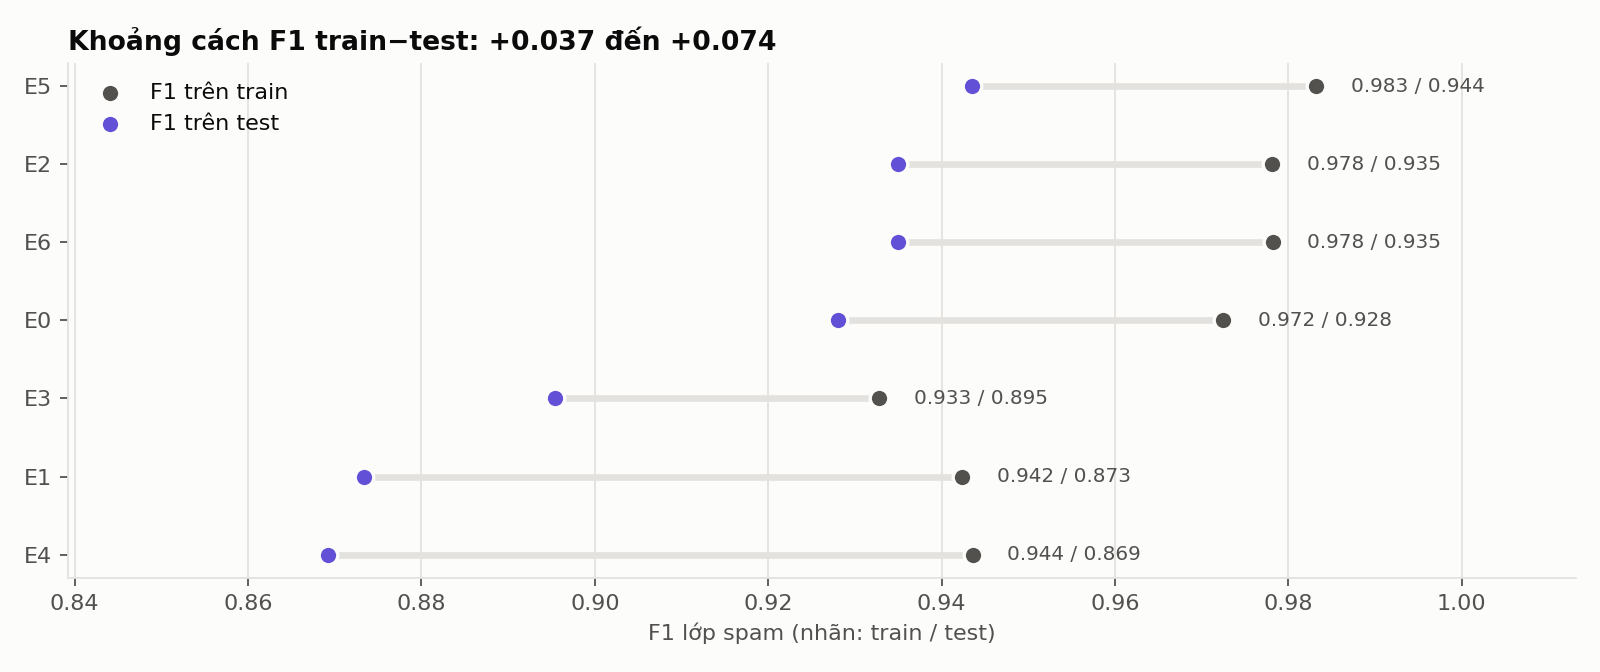
\includegraphics[width=0.95\textwidth]{images/viz_6_overfitting_check.png}
    \caption{Khoảng cách F1 giữa tập huấn luyện và tập kiểm tra}
    \label{fig:overfit}
    \Nguon{Nhóm xây dựng từ kết quả thí nghiệm}
\end{figure}

\section{Độ nhạy theo tham số và thí nghiệm đối chứng}
\label{sec:nhay-tham-so}

Do các thí nghiệm E0--E6 thay đổi nhiều yếu tố cùng lúc, nhóm bổ sung một chuỗi thí nghiệm \textit{thay đổi từng yếu tố một}, đo bằng CV F1 trên tập huấn luyện (không chạm vào tập kiểm tra). Cấu hình nền là cấu hình của E5 (token hóa, TF-IDF $(1,2)$-gram, \texttt{min\_df}=2, $\alpha=0{,}1$), trừ khi nêu khác.

\begin{table}[H]
\centering
\caption{Độ nhạy của CV F1 theo từng yếu tố (cấu hình nền E5; $\alpha$ cố định 0,1 trừ dòng khảo sát $\alpha$)}
\label{tab:nhay}
\begin{tabular}{|p{4.4cm}|p{5.2cm}|c|}
\hline
\textbf{Yếu tố} & \textbf{Giá trị} & \textbf{CV F1} \\
\hline
\multirow{4}{4.4cm}{Biểu diễn và n-gram (\texttt{min\_df}=2)}
 & BoW, unigram & 0,9469 \\
\cline{2-3}
 & BoW, $(1,2)$-gram & 0,9405 \\
\cline{2-3}
 & TF-IDF, unigram & 0,9439 \\
\cline{2-3}
 & TF-IDF, $(1,2)$-gram & 0,9425 \\
\hline
\multirow{3}{4.4cm}{\texttt{min\_df} (TF-IDF, bigram)}
 & 1 & 0,9472 \\
\cline{2-3}
 & 2 & 0,9425 \\
\cline{2-3}
 & 5 & 0,9366 \\
\hline
\multirow{2}{4.4cm}{\texttt{max\_df}}
 & 0,9 & 0,9425 \\
\cline{2-3}
 & 1,0 & 0,9425 \\
\hline
\multirow{5}{4.4cm}{Làm mượt $\alpha$ (TF-IDF, bigram)}
 & 0,01 & 0,9436 \\
\cline{2-3}
 & 0,05 & 0,9427 \\
\cline{2-3}
 & 0,1 & 0,9425 \\
\cline{2-3}
 & 0,5 & 0,9123 \\
\cline{2-3}
 & 1,0 & 0,8597 \\
\hline
\end{tabular}
\Nguon{Nhóm thực nghiệm; kết quả trên tập huấn luyện bằng CV phân tầng 5 fold}
\end{table}

\textbf{Phát hiện 1: $\alpha$ là yếu tố có tác động lớn nhất.} CV F1 giữ ổn định ($\approx0{,}943$) với $\alpha\le0{,}1$ rồi sụt mạnh còn 0,9123 ở $\alpha=0{,}5$ và 0,8597 ở $\alpha=1{,}0$. Cơ chế: vector TF-IDF đã chuẩn hóa $L_2$ nên mỗi thành phần $\le1$ và tổng $N_{wc}$ trên một từ nhỏ so với số đếm thô của BoW; một $\alpha$ cố định (ví dụ 1,0) khi đó ``đè bẹp'' tín hiệu của các từ hiếm nhưng quyết định như \textit{prize} hay \textit{claim}, đẩy mô hình về lớp đa số. Đây cũng là lời giải thích hợp lý cho Recall thấp của E1 ($\alpha=0{,}5$) và cho thấy $\alpha$ mặc định của BoW \textit{không chuyển thẳng} sang TF-IDF.

\textbf{Phát hiện 2: không có bằng chứng rằng TF-IDF hay bigram hơn BoW unigram.} Với tham số $\alpha$ phù hợp, bốn tổ hợp biểu diễn/n-gram chỉ chênh nhau trong khoảng 0,9405--0,9469 (biên độ 0,006), nhỏ hơn độ lệch chuẩn khi thay đổi cách chia dữ liệu ($\approx0{,}012$--$0{,}019$, xem Mục~\ref{sec:on-dinh}). Thậm chí BoW unigram có CV F1 nhỉnh nhất. Giả thuyết ban đầu \textbf{H2} (bigram mang thêm thông tin) vì thế \textit{không được kiểm chứng} trên bộ dữ liệu này, một phần vì các từ khóa spam đơn lẻ đã đủ mạnh. Nhóm vẫn giữ cấu hình bigram cho E5 như đã cố định từ trước khi chạy thí nghiệm độ nhạy, và ghi nhận trung thực rằng nó không phải yếu tố tạo khác biệt.

\textbf{Phát hiện 3: \texttt{min\_df}=1 nhỉnh hơn nhẹ, \texttt{max\_df} không có tác dụng.} Giữ cả các n-gram hiếm cho CV F1 cao hơn (0,9472 so với 0,9366 khi \texttt{min\_df}=5), phù hợp với việc nhiều spam chứa các cụm hiếm nhưng đặc trưng. \texttt{max\_df} không thay đổi kết quả vì ít n-gram nào xuất hiện ở trên 90\% văn bản.

\subsection{Thí nghiệm đối chứng về tiền xử lý}

Bảng~\ref{tab:ablation} tách tác động của từng bước làm sạch (cùng vector hóa TF-IDF $(1,2)$-gram, $\alpha=0{,}1$).

\begin{table}[H]
\centering
\caption{Ablation tiền xử lý: CV F1 trên tập huấn luyện}
\label{tab:ablation}
\begin{tabular}{|p{8.6cm}|c|c|}
\hline
\textbf{Cấu hình làm sạch} & \textbf{CV F1} & \textbf{So với E2} \\
\hline
Chỉ chữ thường (E2) & 0,9365 & -- \\
\hline
$+$ bỏ dấu câu & 0,9365 & $0{,}0000$ \\
\hline
$+$ token hóa URL (kèm bỏ dấu câu) & 0,9299 & $-0{,}0066$ \\
\hline
$+$ token hóa tiền (kèm bỏ dấu câu) & 0,9387 & $+0{,}0022$ \\
\hline
$+$ token hóa số (kèm bỏ dấu câu) & 0,9498 & $+0{,}0133$ \\
\hline
Token hóa URL, tiền, số và bỏ dấu câu (E5) & 0,9425 & $+0{,}0060$ \\
\hline
E5 $+$ bỏ stopword & 0,9464 & $+0{,}0099$ \\
\hline
Bỏ dấu câu $+$ bỏ stopword, không token hóa (E6) & 0,9283 & $-0{,}0082$ \\
\hline
\end{tabular}
\Nguon{Nhóm thực nghiệm; E2, E5, E6 trùng với cột CV F1 của Bảng~\ref{tab:ket-qua}}
\end{table}

Các kết luận rút ra, được phát biểu thận trọng:

\begin{itemize}
    \item \textbf{Token hóa số là bước hữu ích nhất} ($+0{,}0133$), nhất quán với EDA (Bảng~\ref{tab:dac-diem}): 76,5\% spam chứa chuỗi từ 5 chữ số trở lên trong khi chỉ 0,1\% ham có. Số điện thoại và đầu số hầu như duy nhất ở mỗi tin, nên nếu không gom về \texttt{numtoken} mô hình không thể khái quát hóa.
    \item \textbf{Token hóa URL đơn lẻ có xu hướng làm giảm} ($-0{,}0066$). Một lý do có thể là bộ nhận diện URL dựa trên biểu thức chính quy sẽ nhận nhầm một số chuỗi như \textit{``co.uk''} trong văn bản thường. Nhóm chưa kiểm chứng riêng nguyên nhân này, vì vậy chỉ nêu như một giả thuyết cần theo dõi.
    \item \textbf{Hiệu quả của việc bỏ stopword không nhất quán về dấu}: làm giảm khi không có token hóa (E6: $-0{,}0082$ so với E2) nhưng làm tăng khi đi cùng token hóa ($+0{,}0039$ so với E5). Với biên độ nhỏ hơn độ biến thiên khi đổi cách chia dữ liệu, kết luận an toàn là \textit{không có bằng chứng bỏ stopword giúp ích}. Điều này phù hợp với giả thuyết \textbf{H3} rằng các từ như \textit{call}, \textit{your} mang tín hiệu, nên không bỏ chúng một cách mặc định.
    \item \textbf{Hiệu ứng cộng gộp}: tổ hợp E5 ($+0{,}0060$) không bằng riêng token hóa số ($+0{,}0133$); các bước tương tác với nhau và không nên chọn theo trực giác ``làm nhiều bước hơn thì tốt hơn''.
\end{itemize}

\textbf{Lưu ý trung thực về lựa chọn E5.} Cấu hình \textit{``chỉ token hóa số''} (CV F1 0,9498) và \textit{BoW unigram} (0,9469) trong các thí nghiệm độ nhạy cho CV F1 cao hơn E5 (0,9425). Cấu hình E5 được định nghĩa và chọn trong bộ thí nghiệm chính E0--E6 \textit{trước khi} chạy phân tích độ nhạy; nhóm không chuyển sang cấu hình khác sau khi nhìn kết quả để tránh tối ưu quá mức trên dữ liệu kiểm định. Ý nghĩa thực tiễn cũng nhỏ: các chênh lệch này nằm trong dải nhiễu của phép đo (Mục~\ref{sec:on-dinh}).

\section{Độ ổn định theo cách chia dữ liệu}
\label{sec:on-dinh}

Tập kiểm tra chỉ có 128 spam nên mỗi tin bị phân loại sai làm F1 thay đổi khoảng 0,4 điểm phần trăm. Để đo độ dao động này, nhóm lặp lại \textit{toàn bộ} quy trình (chia, huấn luyện, kiểm tra) với 10 hạt giống khác nhau $\text{seed}\in\{0,\dots,9\}$.

\begin{table}[H]
\centering
\caption{F1 của lớp spam trên tập kiểm tra qua 10 lần chia ngẫu nhiên}
\label{tab:on-dinh}
\begin{tabular}{|c|c|c|c|c|}
\hline
\textbf{ID} & \textbf{Trung bình} & \textbf{Độ lệch chuẩn} & \textbf{Nhỏ nhất} & \textbf{Lớn nhất} \\
\hline
E5 & 0,9484 & 0,0140 & 0,9256 & 0,9721 \\
\hline
E2 & 0,9428 & 0,0187 & 0,9076 & 0,9636 \\
\hline
E0 & 0,9411 & 0,0124 & 0,9180 & 0,9603 \\
\hline
E6 & 0,9357 & 0,0125 & 0,9076 & 0,9558 \\
\hline
E3 & 0,9040 & 0,0120 & 0,8841 & 0,9218 \\
\hline
E1 & 0,8657 & 0,0156 & 0,8364 & 0,8821 \\
\hline
E4 & 0,8382 & 0,0236 & 0,7951 & 0,8714 \\
\hline
\end{tabular}
\Nguon{Nhóm thực nghiệm (lệnh \texttt{python -m spam\_filter viz --stability})}
\end{table}

\begin{figure}[H]
    \centering
    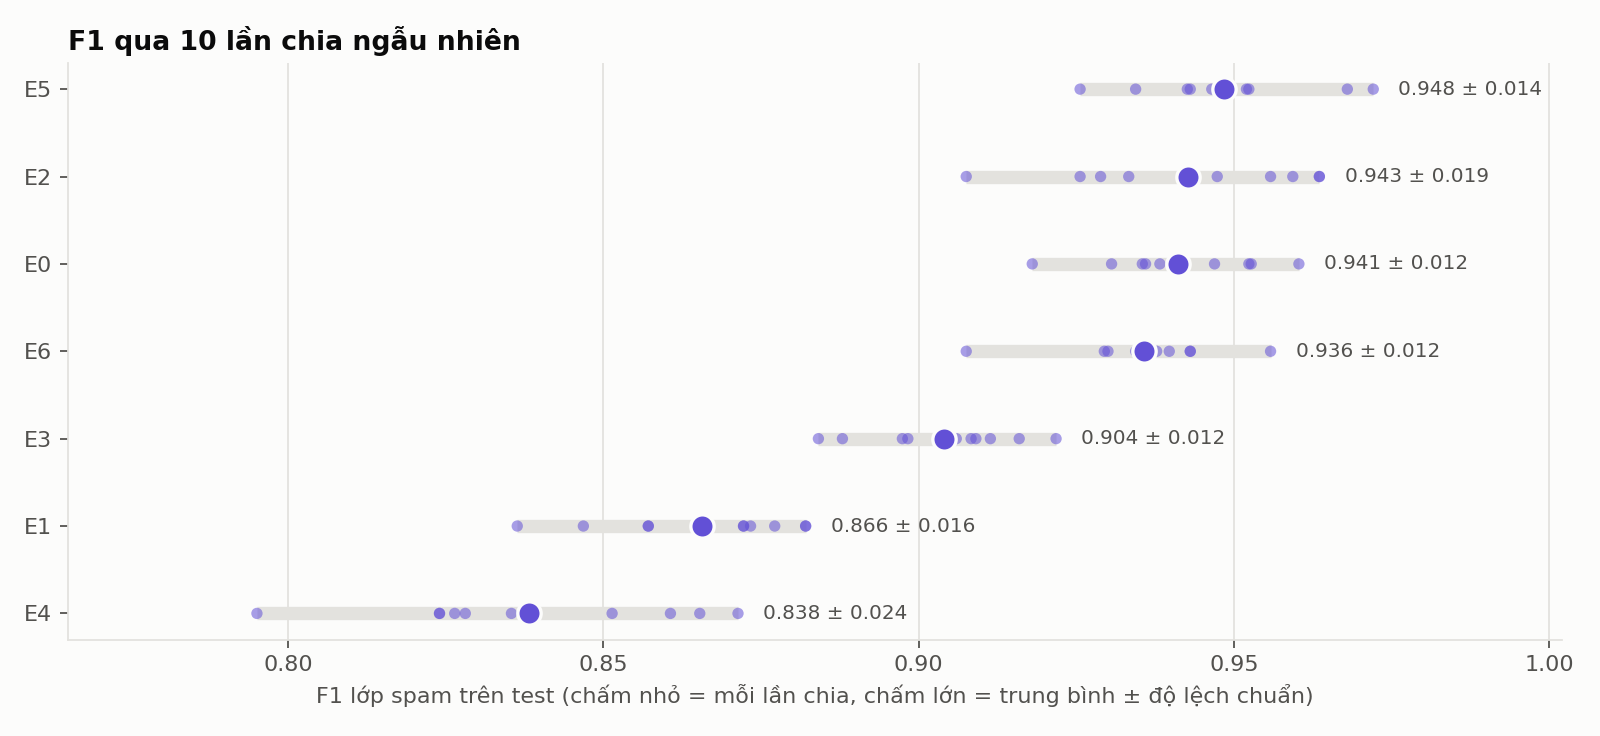
\includegraphics[width=0.95\textwidth]{images/viz_8_f1_stability.png}
    \caption{Phân bố F1 trên tập kiểm tra qua 10 lần chia ngẫu nhiên}
    \label{fig:on-dinh}
    \Nguon{Nhóm xây dựng từ kết quả thí nghiệm}
\end{figure}

Có hai điều rút ra. Thứ nhất, độ lệch chuẩn của F1 là 0,012--0,024, \textbf{lớn hơn khoảng cách giữa E5, E2, E0 và E6} (biên độ trung bình 0,013). Nói cách khác \textit{một lần chia duy nhất không đủ để xếp hạng} nhóm NB. So sánh theo cặp trên cùng cách chia cho thấy E5 hơn E0 trung bình $+0{,}0073\pm0{,}0080$ (thắng 7 trên 10 lần, hòa 1) và hơn E2 trung bình $+0{,}0056\pm0{,}0104$ (thắng 5, hòa 3); xu hướng có lợi cho E5 nhưng với 10 lần chia không độc lập (các tập huấn luyện chồng lấn), nhóm \textbf{không tuyên bố ý nghĩa thống kê}. Thứ hai, khoảng cách giữa họ NB và K-NN/Cây ($0{,}04$--$0{,}11$) vượt xa độ dao động và xuất hiện ở mọi lần chia, nên kết luận này \textit{đáng tin}. E1 thấp hơn E0 ở 10/10 lần chia (trung bình $-0{,}075$), khẳng định vấn đề của $\alpha=0{,}5$ không phải do may rủi.

\section{Đường cong học}

Đường cong học của E5 (Hình~\ref{fig:learning-curve}) cho thấy F1 kiểm định tăng nhanh đến khoảng 2\,000 mẫu huấn luyện rồi gần như đi ngang quanh 0,94; khoảng cách giữa điểm huấn luyện (0,984) và điểm kiểm định (0,943) còn khoảng 0,04. Hai điều này đồng nhất: mô hình có phương sai vừa phải và việc \textit{chỉ thêm dữ liệu cùng loại} sẽ cho lợi ích giảm dần; muốn cải thiện đáng kể cần thông tin mới (dữ liệu spam hiện đại hơn hoặc đặc trưng tốt hơn), phù hợp với các lỗi quan sát được ở Chương~6.

\begin{figure}[H]
    \centering
    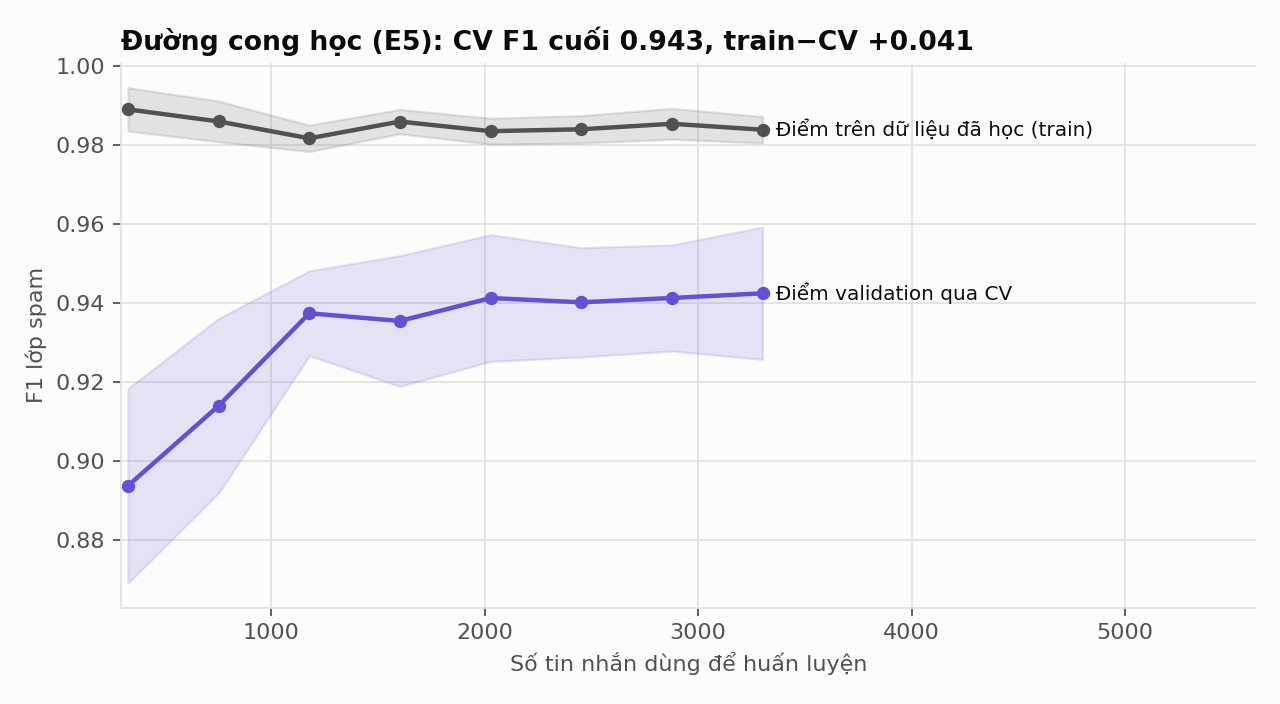
\includegraphics[width=0.9\textwidth]{images/viz_9_learning_curve.png}
    \caption{Đường cong học của E5 (F1 lớp spam theo số mẫu huấn luyện)}
    \label{fig:learning-curve}
    \Nguon{Nhóm xây dựng bằng lệnh \texttt{python -m spam\_filter check}}
\end{figure}

\section{Kiểm tra rò rỉ dữ liệu và học thuộc}
\label{sec:sanity}

Một kết quả F1 trên 0,94 cho bài toán lọc spam dễ khiến người đọc nghi ngờ. Nhóm vì vậy cài đặt chín phép kiểm tra tự động cho mô hình E5 (Bảng~\ref{tab:sanity}).

\begin{table}[H]
\centering
\caption{Kết quả các phép kiểm tra rò rỉ, học thuộc và baseline đơn giản (mô hình E5)}
\label{tab:sanity}
\small
\begin{tabular}{|p{6.1cm}|p{4.6cm}|c|}
\hline
\textbf{Phép kiểm tra} & \textbf{Kết quả} & \textbf{Trạng thái} \\
\hline
A1. Tin trùng chính xác giữa train và test & 0 (yêu cầu $=0$) & OK \\
\hline
A2. Trùng sau chuẩn hóa chữ hoa/thường, dấu câu & 8 (yêu cầu $=0$) & Lưu ý \\
\hline
A3. Tin test có bản gần giống (cosine $\ge0{,}8$) trong train & 65 tin (6,3\%) & OK \\
\hline
A4. F1 trên tin ``mới'' (không có bản gần giống) & 0,912 (toàn test 0,944; giảm 0,031) & OK \\
\hline
A5. Xáo trộn nhãn train rồi đo trên test (5 lần) & F1 trung bình 0,105 & OK \\
\hline
B1. Chênh lệch F1 train $-$ test & $0{,}983-0{,}944=0{,}040$ & OK \\
\hline
B2. F1 CV (train) so với test & 0,943 so với 0,944 & OK \\
\hline
C1. Baseline chỉ dùng độ dài và số chữ số & F1 0,886 (mô hình hơn 0,057) & OK \\
\hline
C2. Đoán ngẫu nhiên theo tỉ lệ lớp & F1 0,083 & OK \\
\hline
\end{tabular}
\Nguon{Nhóm thực nghiệm (lệnh \texttt{python -m spam\_filter check}); kết quả: 8 OK, 1 lưu ý, 0 lỗi}
\end{table}

Diễn giải theo từng nhóm:

\begin{itemize}
    \item \textbf{Rò rỉ (A).} Không có tin trùng chính xác giữa hai tập. Tám tin trùng \textit{sau khi chuẩn hóa} (khác nhau chỉ ở chữ hoa/dấu câu) là một ``lưu ý'' nhỏ, chiếm dưới 1\% tập kiểm tra. Khi chỉ xét các tin test \textit{không} có bản gần giống trong train (A4), F1 giảm 0,031 xuống 0,912, nghĩa là một phần nhỏ điểm số đến từ các tin gần trùng nhưng phần lớn vẫn là khả năng khái quát hóa thực. Phép xáo trộn nhãn (A5) cho F1 xấp xỉ 0,105, tức mô hình trở về mức đoán mò khi nhãn mất ý nghĩa, một chứng cứ mạnh rằng pipeline \textit{không} ``nhìn trộm'' nhãn.
    \item \textbf{Học thuộc (B).} Chênh lệch train--test (0,040) thấp, và CV trên train (0,943) khớp tập test (0,944).
    \item \textbf{Bài toán có thật sự khó không (C).} Baseline chỉ dùng độ dài và số chữ số đã đạt F1 0,886, nên bài toán trên corpus này \textit{tương đối dễ}: một phần lớn tín hiệu nằm ở đặc điểm cấu trúc. Mô hình NB hơn baseline đơn giản này 0,057 F1; đó là mức cải thiện có thật nhưng khiêm tốn, cần được nhìn nhận khi đánh giá ``độ khó'' của bài toán.
\end{itemize}

Một cảnh báo quan trọng: các phép kiểm tra này loại trừ rò rỉ \textit{trong nội bộ corpus}, không loại trừ \textit{thiên lệch nguồn} (ham chủ yếu từ Singapore, spam từ Vương quốc Anh; xem Mục~1.4). Mô hình có thể một phần dựa vào dấu hiệu nguồn gốc như phương ngữ.

\section{Ảnh hưởng của ngưỡng quyết định}

Mặc định mô hình gọi một tin là spam khi $P(\text{spam}\mid d)\ge0{,}5$. Vì chi phí của FP và FN khác nhau (Mục~1.6), nhóm khảo sát việc đổi ngưỡng cho E5 (Bảng~\ref{tab:nguong}, Hình~\ref{fig:nguong}).

\begin{table}[H]
\centering
\caption{Precision, Recall, F1 và số lỗi của E5 theo ngưỡng quyết định (tập kiểm tra)}
\label{tab:nguong}
\begin{tabular}{|c|c|c|c|c|c|}
\hline
\textbf{Ngưỡng} & \textbf{Precision} & \textbf{Recall} & \textbf{F1} & \textbf{FP} & \textbf{FN} \\
\hline
0,3 & 0,9528 & 0,9453 & 0,9490 & 6 & 7 \\
\hline
0,4 & 0,9754 & 0,9297 & 0,9520 & 3 & 9 \\
\hline
\textbf{0,5 (mặc định)} & 0,9750 & 0,9141 & 0,9435 & 3 & 11 \\
\hline
0,6 & 0,9912 & 0,8828 & 0,9339 & 1 & 15 \\
\hline
0,7 & 0,9912 & 0,8750 & 0,9295 & 1 & 16 \\
\hline
0,8 & 0,9910 & 0,8594 & 0,9205 & 1 & 18 \\
\hline
0,9 & 0,9907 & 0,8359 & 0,9068 & 1 & 21 \\
\hline
\end{tabular}
\Nguon{Nhóm thực nghiệm}
\end{table}

\begin{figure}[H]
    \centering
    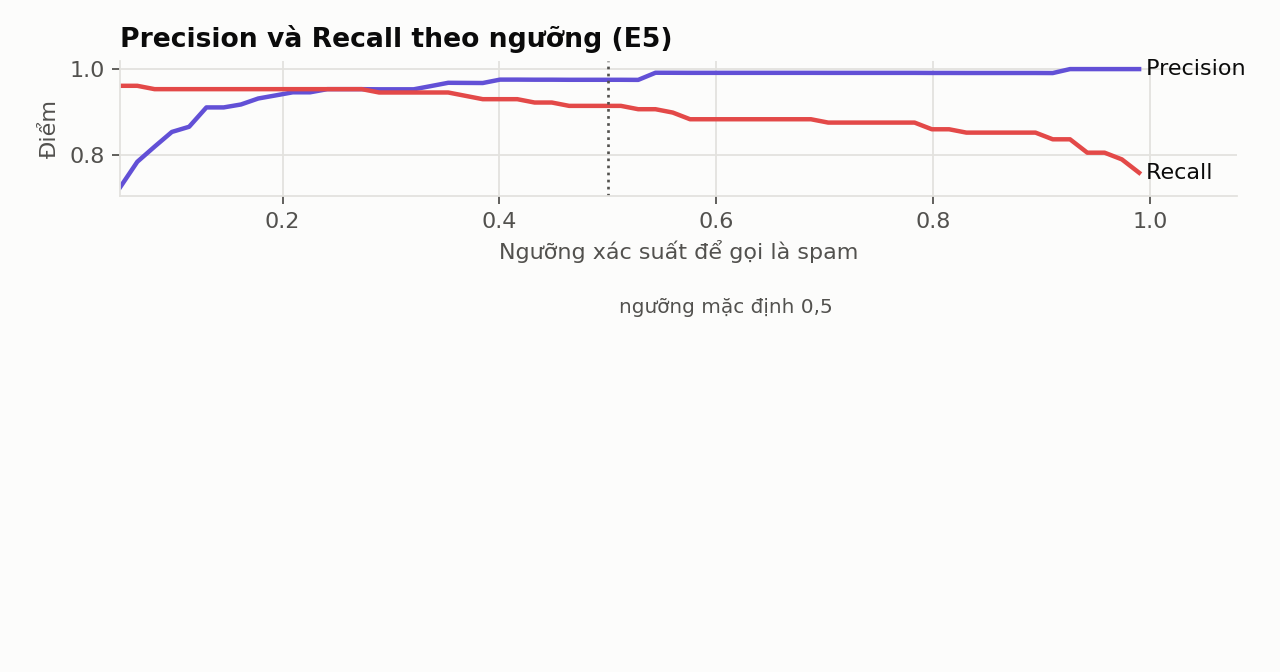
\includegraphics[width=0.85\textwidth]{images/viz_7_threshold_tradeoff.png}
    \caption{Đường Precision và Recall của E5 theo ngưỡng xác suất}
    \label{fig:nguong}
    \Nguon{Nhóm xây dựng từ kết quả thí nghiệm}
\end{figure}

Tăng ngưỡng từ 0,5 lên 0,6 giảm FP từ 3 xuống 1 nhưng làm FN tăng từ 11 lên 15; từ 0,6 trở đi hầu như không còn giảm được FP nào nữa (vẫn còn 1 tin ham bị chặn) trong khi FN tiếp tục tăng. Điều này cho thấy tin ham còn sót lại là tin mô hình \textit{rất tự tin} nhầm lẫn, ngưỡng không giải quyết được. \textbf{Lưu ý phương pháp}: các giá trị ở Bảng~\ref{tab:nguong} được đọc trên tập kiểm tra nên chỉ mang tính \textit{mô tả}; nếu triển khai thật, ngưỡng phải được chọn bằng CV trên tập huấn luyện hoặc một tập validation riêng, rồi mới đánh giá một lần trên tập test.
